\section{UC\#3: isolation of vulnerability-prone components}\label{appendix:seapp_uc3}

In this use case we show how to confine a set of components, which
rely on a high performance native library written in C to perform some
task. Our goal is to demonstrate that the context running the native
library code is prevented to access the network, even when the
permissions {\em INTERNET} and {\em ACCESS\textunderscore
  NETWORK\textunderscore STATE} are granted to the app sandbox.

\begin{figure}[h]
  \centering
  \subfloat{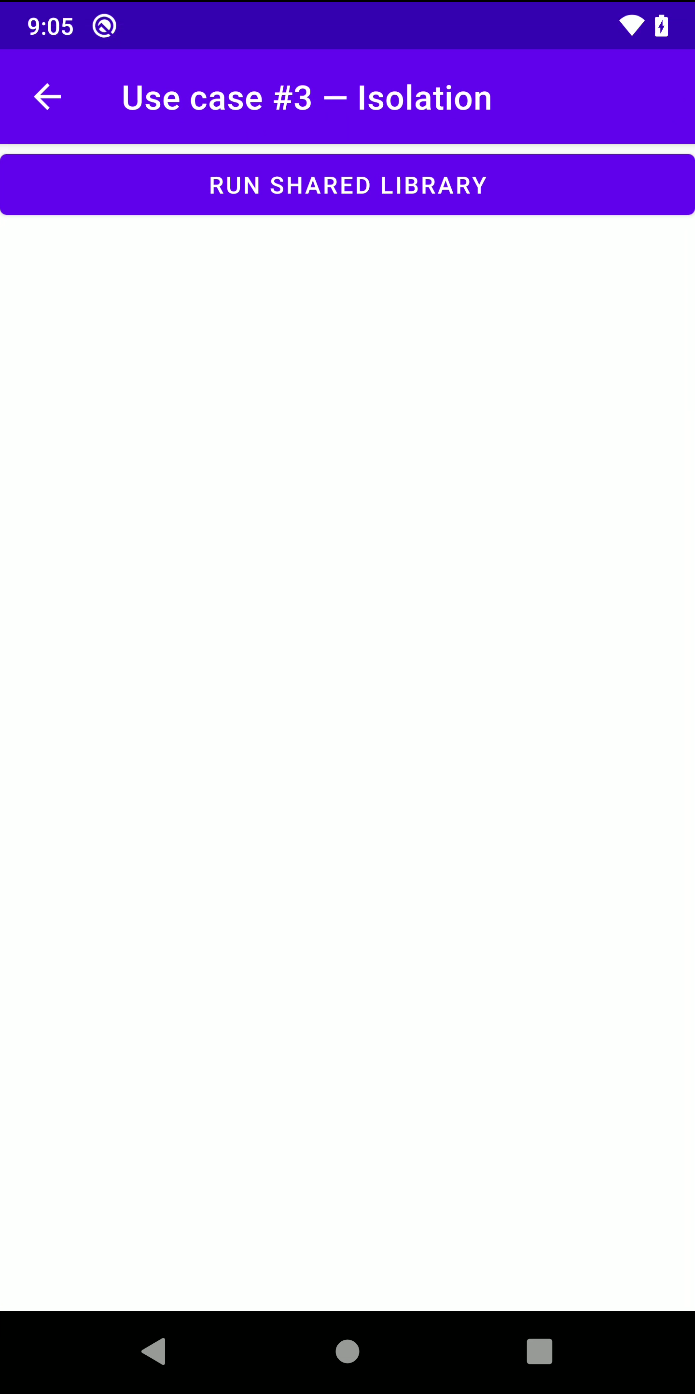
\includegraphics[width=0.3\textwidth]{chapters/seapp/figs/ae/uc31.png}}
  \hfill
  \subfloat{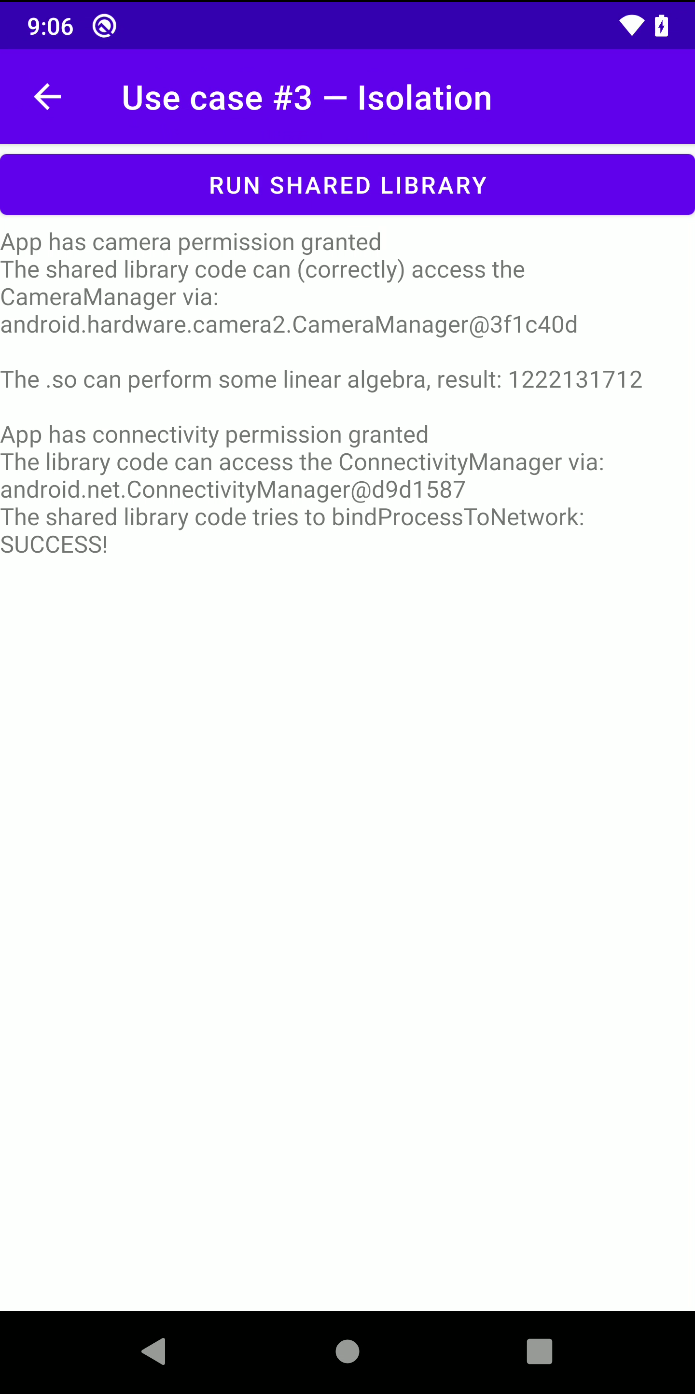
\includegraphics[width=0.3\textwidth]{chapters/seapp/figs/ae/uc32.png}}
  \hfill
  \subfloat{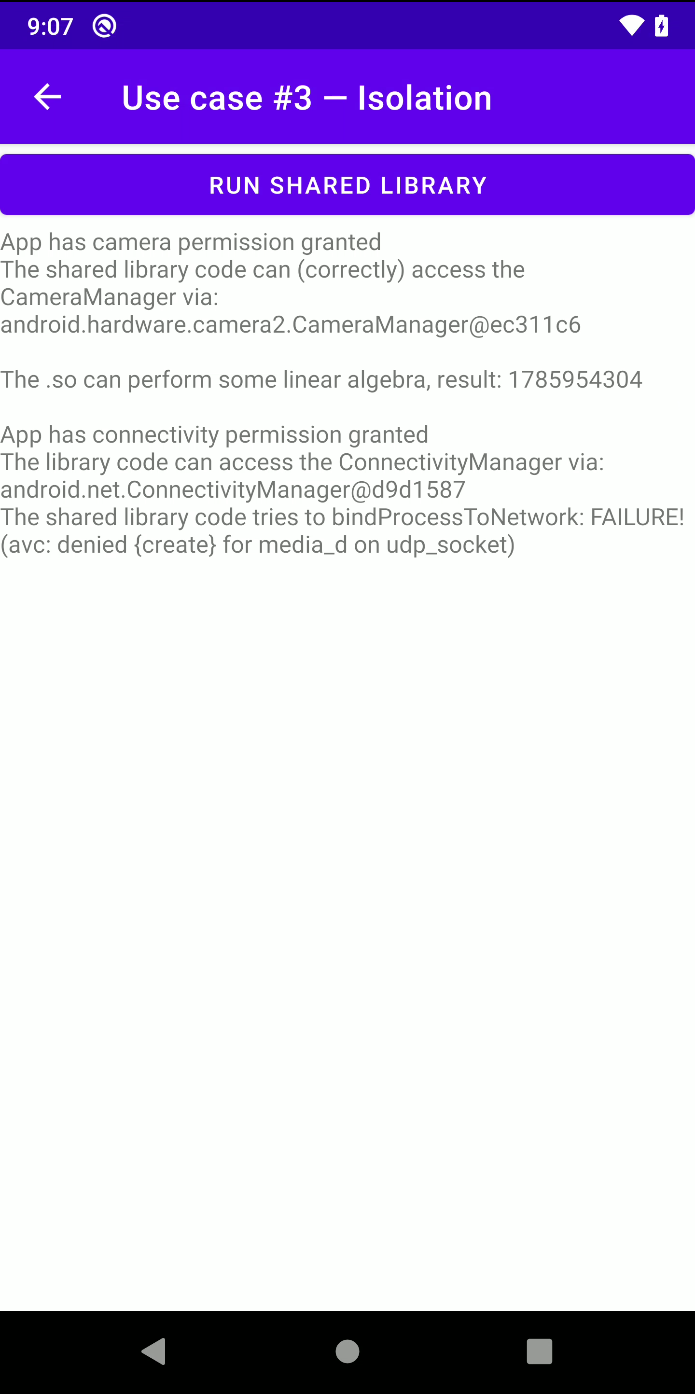
\includegraphics[width=0.3\textwidth]{chapters/seapp/figs/ae/uc33.png}}
  \caption{\label{fig:seapp_uc3_views} UC\#3 views (initiation, exploitation, and mitigation)}
\end{figure}

The native library is invoked by {\em UseCase3Activity}
(Figure~\ref{fig:seapp_uc3_views}a), which, according to line 4 in the
\seappcontexts, is executed in a process labeled with {\tt media\_d}
by {\em Zygote}.  The call to the library is performed via JNI. Its
job is to connect to the {\em camera\textunderscore service} and take
a picture.  Since the app is granted the {\em CAMERA} permission, the
native library code (legitimately, line 60 in the \sepolicy) connects
to the {\tt CameraManager}.

Since the native library performs image processing, we do not want it
to access the network. However, the permissions {\em INTERNET} and
{\em ACCESS\textunderscore NETWORK\textunderscore STATE} are granted
to the app, as they are required by the Ads framework.  Thus, when the
policy module is not available, the native library can connect to the
{\tt ConnectivityManager} and successfully bind the current process to
the network (Figure~\ref{fig:seapp_uc3_views}b).  Instead, when the
policy module is enforced by SEApp, since {\tt media\_d} was granted
only the basic app permissions (line 11 in \sepolicy), the connection
to the network is forbidden (Figure~\ref{fig:seapp_uc3_views}c).  This
happens because binding a process to the network is associated with
opening a network socket, an operation not permitted by \sel without
the required permissions. The following denial is written to the
system log: {\em denied {\tt create} on {\tt udp\textunderscore
    socket} to {\tt media\textunderscore d} domain}
(Figure~\ref{fig:seapp_uc3_logcat}).

\begin{figure}[h]
  \centering
  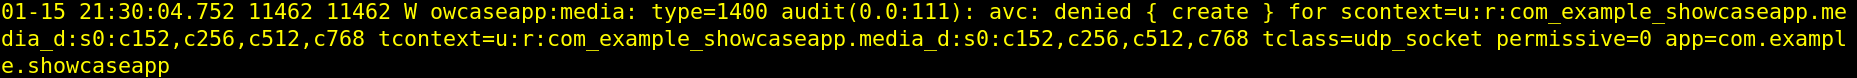
\includegraphics[width=\textwidth]{chapters/seapp/figs/ae/uc35.png}
  \caption{\label{fig:seapp_uc3_logcat}  UC\#3 \sel denial message in the system log}
\end{figure}      

This use case, besides showing how SEApp confines a native library,
also demonstrates the power and simplicity of the macro, as adding the
line {\tt (call md\textunderscore netdomain (media\textunderscore d))}
to the policy module grants to {\tt media\textunderscore d} the needed
permissions to access the network.  The application developer is thus
not required to know or understand the internal \sel policy in order
to leverage this functionality.

The isolation properties introduced by \seapp applies also to other
common security problems presented
in~\cite{seapp_common_play_protect_vulnerabilites}. Just to mention
one, \seapp can mitigate the impact of incorrect sandboxing of a
scripting language.

%%% Local Variables: 
%%% mode: latex
%%% TeX-master: "../../../../main.tex"
%%% reftex-default-bibliography: "../../../../bib/biblio.bib"
%%% End: